\subsection{Dependency Inversion Principle}
    This principle states that higher level modules should not depend on 
    the low-level modules but they should both depend on abstractions. If one class 
    knows explicitly about the design and implementation of another class,
    the change made to one class could break the other classes. This could
    create a series of rippling effects to break the program and DI can help avoid this. Figure
    \ref{fig:DIExample} gives us an overview of the principle.

    \begin{figure}[htbp!]
        \centering 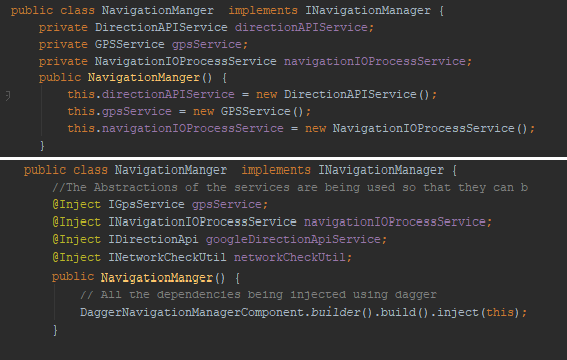
\includegraphics{grafiken/di_compare.png}
        \caption{Comparision of code with(bottom) and without Dependency injection(top)}
        \label{fig:DIComparision}
    \end{figure}

    \par
        Dependency Inversion will be achieved in this module with the help of a dependency
        injector Dagger \cite{SquareDagger} 
        see Appendix \ref{appendix:dagger}. 
        This framework is responsible for creating and managing the 
        objects and injecting them to the required
        class. 
        Figure \ref{fig:DIComparision} shows a snippet of a class 
        NavigationManager one without DI and one with DI.
        It can be seen that in the code which is not using 
        DI the dependencies are tightly coupled because all the
        dependencies are handled inside the class NavigationManager.
        Using DI the object creation is being handled by the
        framework which would lead to decoupling of these dependencies.

    
        